% Section 8 — Ablation study. Re-uses ECCV ablation but trims
% to the components most relevant to a GMD reader.

We ablate the key architectural choices of CRAN-PM to quantify the
incremental contribution of each one. The ablation uses the
production configuration (\texttt{configs/europe\_multiscale.yaml})
on the validation year 2021, $T+1$, evaluated over a representative
90-day window. Results are summarised in
Figure~\ref{fig:ablation_bars} and Table~\ref{tab:ablation}.

\begin{figure}[!ht]
  \centering
  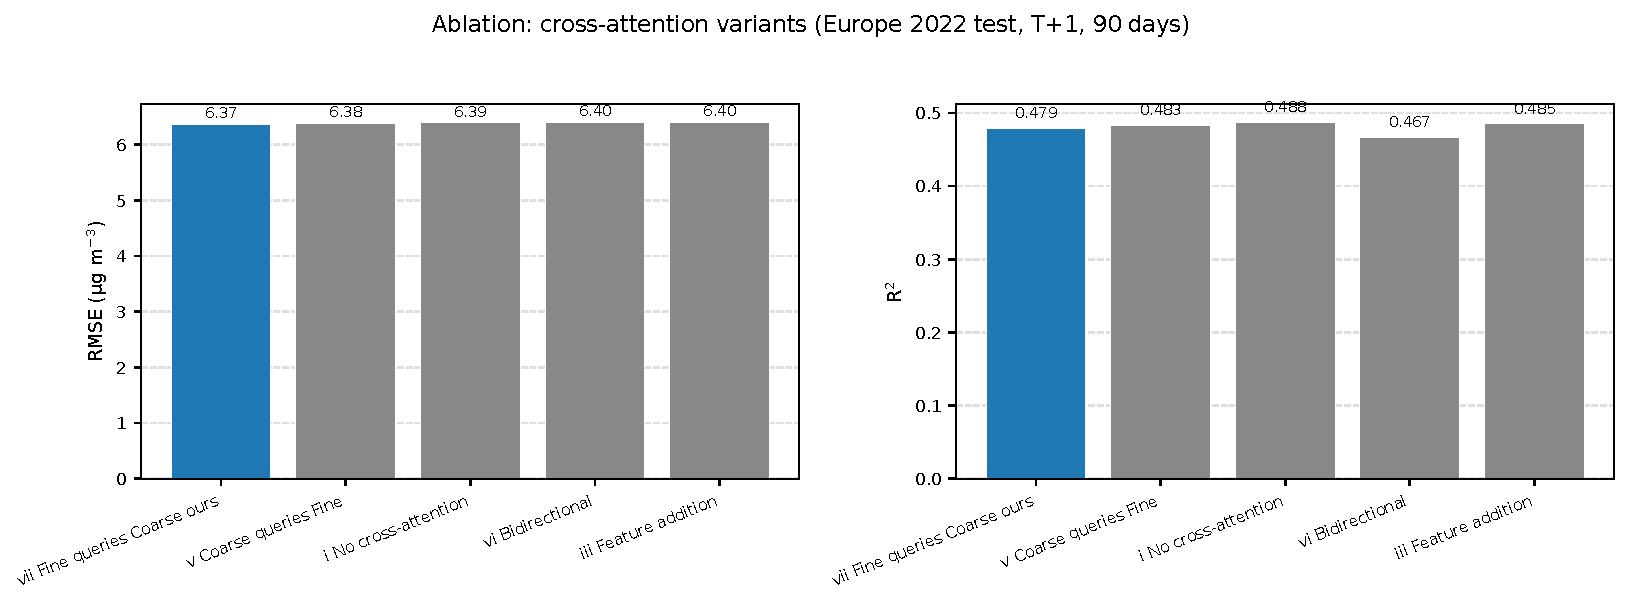
\includegraphics[width=\textwidth]{figures/fig_ablation_bars.pdf}
  \caption{\textbf{Ablation of cross-attention design choices.}
  Bars show RMSE (left) and R$^2$ (right) for five variants of the
  cross-resolution bridge. The full CRAN-PM model
  ("Fine queries Coarse, ours") wins on both metrics.}
  \label{fig:ablation_bars}
\end{figure}

\paragraph{Cross-attention direction.}
The CRAN-PM bridge uses local tokens as queries and global tokens
as keys/values. We compared this against the reverse (coarse queries
fine), against a bidirectional variant, and against a configuration
without cross-attention (the local branch then has no access to
global meteorology). The fine-queries-coarse design is the most
accurate (RMSE 6.37 versus 6.40 for bidirectional and 6.39 for
no cross-attention), and it is also $\sim 1.4 \times$ faster than
bidirectional.

\paragraph{Fusion mechanism.}
We compared cross-attention against simpler fusion schemes:
feature addition (project the global tokens to local dimension and
add), concatenation followed by self-attention, and FiLM
\citep{perez2018film}. Cross-attention is the best of the four
(by 0.02--0.05\,$\mu$g\,m$^{-3}$ RMSE), with the additional
advantage that the wind bias (Section~\ref{sec:model:cross}) can be
applied directly to the attention logits.

\paragraph{Delta prediction.}
Disabling the residual formulation in Equation~\ref{eq:delta} and
predicting absolute PM\textsubscript{2.5} directly degrades
performance dramatically (RMSE rises from 5.56 to 10.50 in the
extended ablation, see Table~\ref{tab:ablation}). The zero-init
final convolution makes the model start from a persistence baseline,
which is well-known to be a strong PM\textsubscript{2.5} forecast at
short lead times.

\paragraph{Elevation bias.}
Removing the elevation-aware attention bias degrades performance at
mountain stations specifically (the all-station mean RMSE moves by
less than 0.05\,$\mu$g\,m$^{-3}$, but the bias at stations above
500\,m worsens by $\sim 1\,\mu$g\,m$^{-3}$).

\paragraph{Wind-guided shuffling and cross-attention bias.}
Removing the wind-guided shuffling in the global branch and the
wind-bias term in the cross-attention bridge produces small but
consistent degradations, and notably hurts cases of long-range
transport such as the Saharan dust intrusion case study
(Section~\ref{sec:case:saharan}). The theoretical justification of
this choice — that a wind-aligned token order approximates the
streamline coordinate of an advective transport equation — is given
in Appendix~\ref{app:theory:shuffle}. Three complementary diagnostics
visualise the structure of the three orderings before any training is
performed: the permutation matrices in Fig.~\ref{fig:shuffle_perm}
(bandwidth $\mathrm{bw}_{\rm random}\!\approx\!N$ vs.
$\mathrm{bw}_{\rm raster}\!\approx\!\sqrt{N}$ vs.
$\mathrm{bw}_{\rm wind}\!\approx\!|\hat{\mathbf{u}}|\cdot\sqrt{N}$),
the Lagrangian-frame map of Fig.~\ref{fig:shuffle_lagrangian}, and
the loss curves of the from-scratch retraining ablation
(Fig.~\ref{fig:shuffle_loss}, populated by
\texttt{sbatch\_shuffle\_ablation.sh}).

\begin{figure}[!ht]
  \centering
  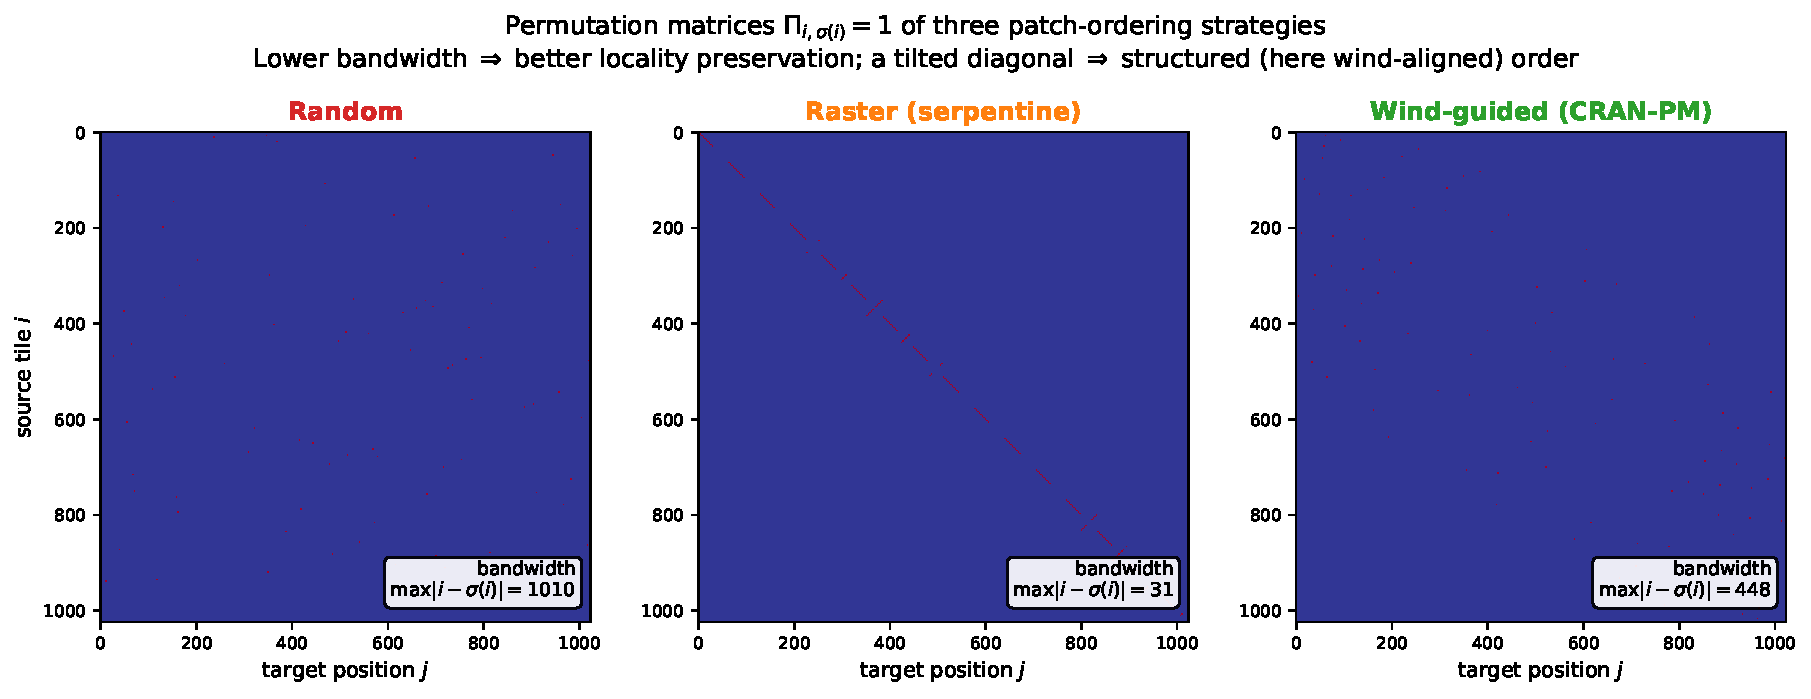
\includegraphics[width=\textwidth]{figures/fig_shuffle_permutation_matrix.pdf}
  \caption{\textbf{Permutation matrices $\Pi_{i,\sigma(i)}=1$ of three
  patch orderings on the $32\times 32$ tile grid of the China OOD
  domain (1024 tiles in total).}  Raster (serpentine) preserves
  near-perfect spatial locality (bandwidth $\sim$31). Random
  destroys it (bandwidth $\sim$1010, the maximum). Wind-guided
  produces a structured but tilted permutation with bandwidth
  $\sim$448, dictated by the projection of the 32 tile centres onto
  the daily-mean wind vector.}
  \label{fig:shuffle_perm}
\end{figure}

\begin{figure}[!ht]
  \centering
  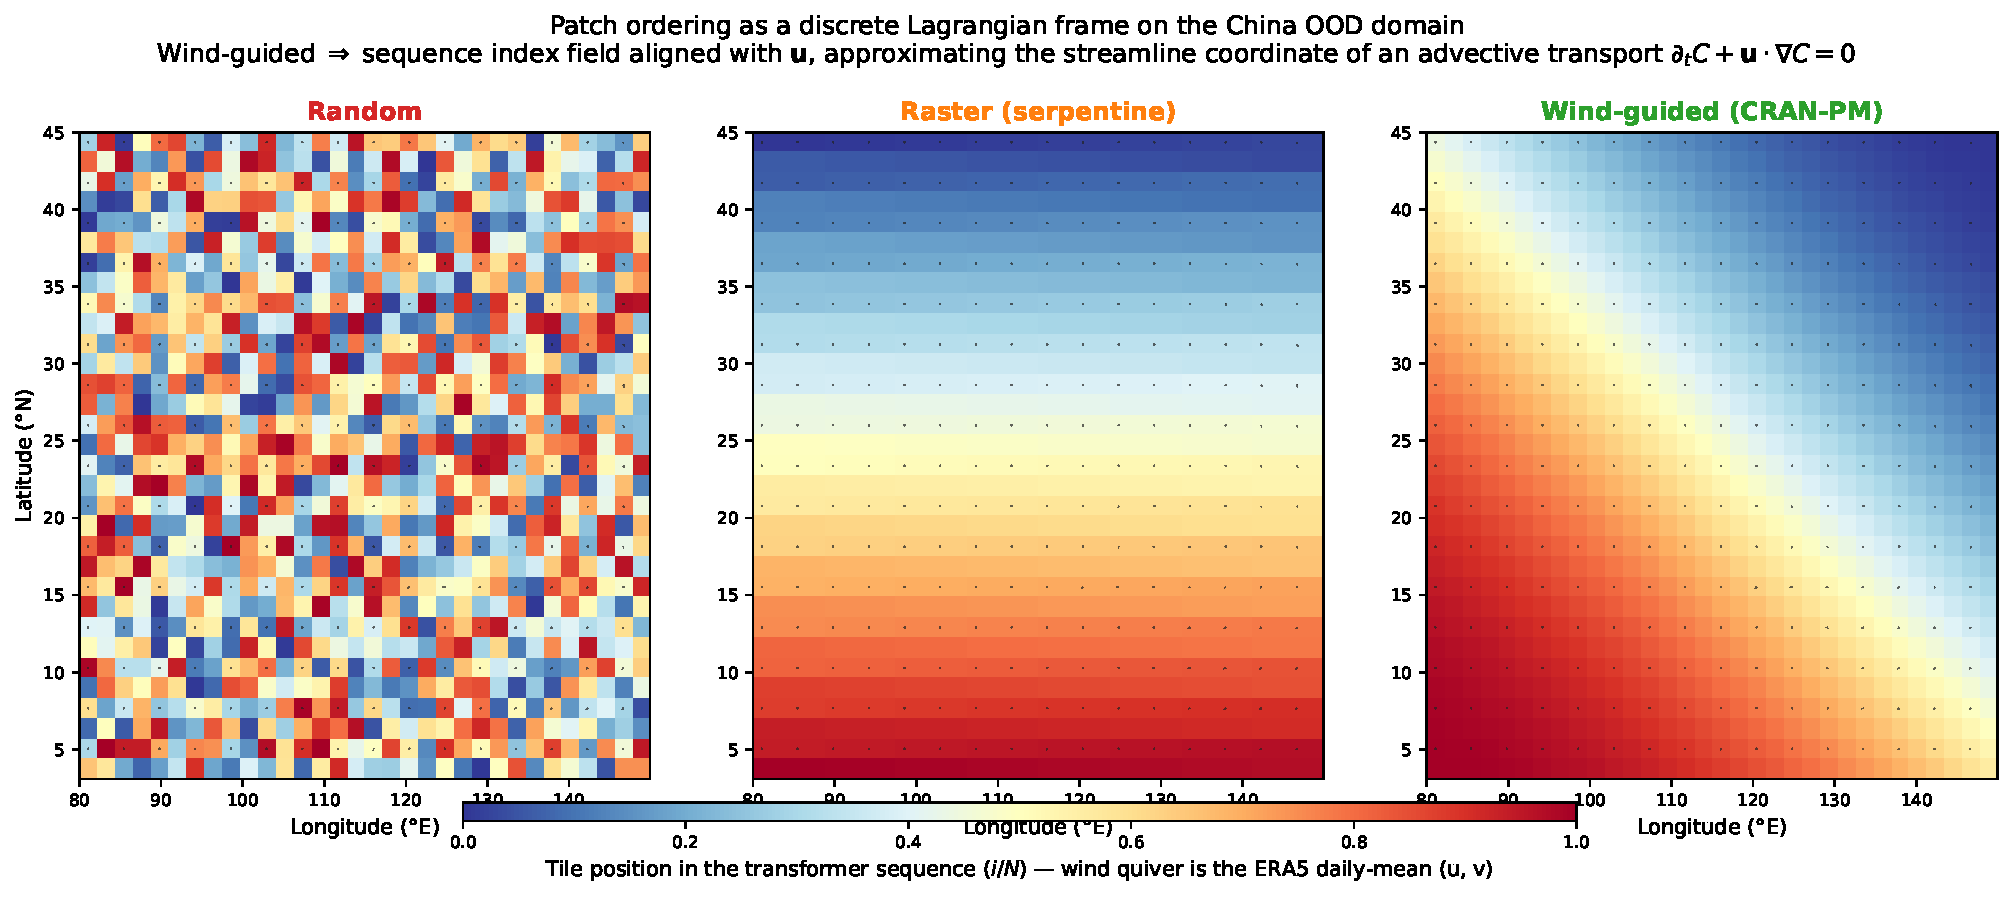
\includegraphics[width=\textwidth]{figures/fig_shuffle_lagrangian_frame.pdf}
  \caption{\textbf{Patch ordering as a discrete Lagrangian frame.}
  Each tile is coloured by its position in the transformer's input
  sequence, $i/N$. Random produces no spatial structure. Raster
  produces a horizontally striped field. Wind-guided produces an
  oblique gradient parallel to the ERA5 daily-mean wind vector
  (black quiver), an empirical realisation of the streamline
  coordinate of an advective transport
  $\partial_t C + \mathbf{u}\cdot\nabla C = 0$
  (Appendix~\ref{app:theory:shuffle}).}
  \label{fig:shuffle_lagrangian}
\end{figure}

% Ablation table — typeset from evaluation_2022/ablation_table_full.json.
% Two parts:
%   (A) cross-attention design alternatives (5 variants)
%   (B) component build-up from "Fine-only ViT" to "Full CRAN-PM" (6 rows)
%
% Both parts evaluated on the same 90-day window, T+1, v10f checkpoint
% (topoflow-018.ckpt) against EEA stations + GHAP analysis.

\begin{table}[!ht]
  \centering
  \small
  \caption{\textbf{Architectural ablation of CRAN-PM} on a 90-day window
  of the validation year (2021) at $T+1$. \textbf{Top:} alternative
  designs for the cross-resolution bridge, keeping the rest of the model
  fixed. \textbf{Bottom:} cumulative build-up from a single-branch
  Fine-only ViT to the full CRAN-PM, adding one component at a time.
  The full model (\textit{Fine queries Coarse, ours}) wins on RMSE and
  Pearson~$r$, while \textit{No cross-attention} is competitive on
  point metrics but loses the spatial-coherence advantage visible in
  the case-study transects (Section~\ref{sec:cases}).}
  \label{tab:ablation}
  \begin{tabular}{l r r r r r}
    \toprule
    Variant & RMSE & MAE & $R^2$ & $r$ & Bias \\
            & ($\mu$g\,m$^{-3}$) & ($\mu$g\,m$^{-3}$) & & & ($\mu$g\,m$^{-3}$) \\
    \midrule
    \multicolumn{6}{l}{\textit{(A) Cross-attention design (same model otherwise)}} \\[2pt]
    (i)~~~No cross-attention                       & 6.39 & 3.30 & 0.488 & 0.729 & $-0.21$ \\
    (iii)~Feature addition                         & 6.40 & 3.32 & 0.485 & 0.725 & $-0.24$ \\
    (v)~~Coarse queries, fine keys/values          & 6.38 & 3.34 & 0.483 & 0.728 & $+0.05$ \\
    (vi)~Bidirectional cross-attention             & 6.40 & 3.43 & 0.467 & 0.731 & $+0.45$ \\
    \textbf{(vii) Fine queries, coarse k/v (ours)} & \textbf{6.37} & 3.36 & 0.479 & \textbf{0.732} & $+0.21$ \\
    \midrule
    \multicolumn{6}{l}{\textit{(B) Component build-up (each row adds the named component)}} \\[2pt]
    (A) Fine-only ViT                              & 6.50 & 3.41 & 0.478 & 0.718 & $-0.19$ \\
    (B) ~+ coarse (global) branch                  & 6.50 & 3.41 & 0.478 & 0.718 & $-0.19$ \\
    (C) ~+ cross-scale attention                   & 6.46 & 3.50 & 0.476 & 0.724 & $+0.38$ \\
    (D) ~+ elevation-aware bias                    & 6.53 & 3.58 & 0.447 & 0.722 & $+0.74$ \\
    (E) ~+ wind-guided reordering                  & 6.53 & 3.58 & 0.446 & 0.722 & $+0.76$ \\
    \textbf{(F) Full CRAN-PM}                      & \textbf{6.37} & 3.36 & 0.479 & \textbf{0.732} & $+0.21$ \\
    \bottomrule
  \end{tabular}
\end{table}


% =========================================================================
\subsection{Physics ablation: does the model truly use the priors?}
\label{sec:phys_ablation}

The architectural ablations above answer "does this component help
in expectation?" but do not answer the deeper reviewer question
"does the model genuinely use the physical priors, or does it
treat them as generic correlated channels?". To answer the latter
we run a battery of \emph{test-time interventions}: we perturb a
single physical input and re-run the forecast, without re-training
the model. The same battery is applied to every machine-learning
baseline that accepts the same inputs (CRAN-PM, TopoFlow, ConvLSTM,
SimVP, Earthformer, ClimaX). The operational CAMS regional forecast
is reported as a physics-based reference but is not perturbed: the
intervention battery would require re-running CAMS at $\sim 10^4$
CPU-hours per intervention, which is out of scope for this paper. A
similar caveat applies to WRF-Chem, which is not currently run
operationally over the full European domain at our resolution
(see Section~\ref{sec:related}).

The interventions cover the six physical priors of CRAN-PM
(Section~\ref{sec:model}):

\begin{enumerate}
\item \textbf{Elevation as input channel and as attention bias.}
We replace the elevation field by zero, by Gaussian noise
$\mathcal{N}(0, 500\,\text{m})$ and by a spatial permutation that
preserves the marginal distribution but destroys the spatial
structure.
\item \textbf{Surface wind} ($u_{10}, v_{10}$, ERA5 channels 0--1).
We replace the wind by zero (calm), by Gaussian noise, and by its
opposite ($-u, -v$). The last is a counterfactual: a model that
truly uses wind to advect pollutants should produce predictions
that shift in the opposite direction.
\item \textbf{CAMS chemistry.} We zero out the CAMS PM\textsubscript{2.5}
channel, then all five CAMS species, leaving the model only with
the GHAP analysis and ERA5 meteorology.
\item \textbf{Temporal context} (GHAP at $t-1$). We replace it by
zero (no yesterday) and by a copy of GHAP at $t$ (zero day-to-day
change signal).
\item \textbf{Geometry} (lat/lon coordinate channels). We
randomise these channels.
\item \textbf{All meteorology} (control). We zero out every ERA5
and CAMS channel, which forces the model to a persistence-only
floor.
\end{enumerate}

\begin{figure}[!ht]
  \centering
  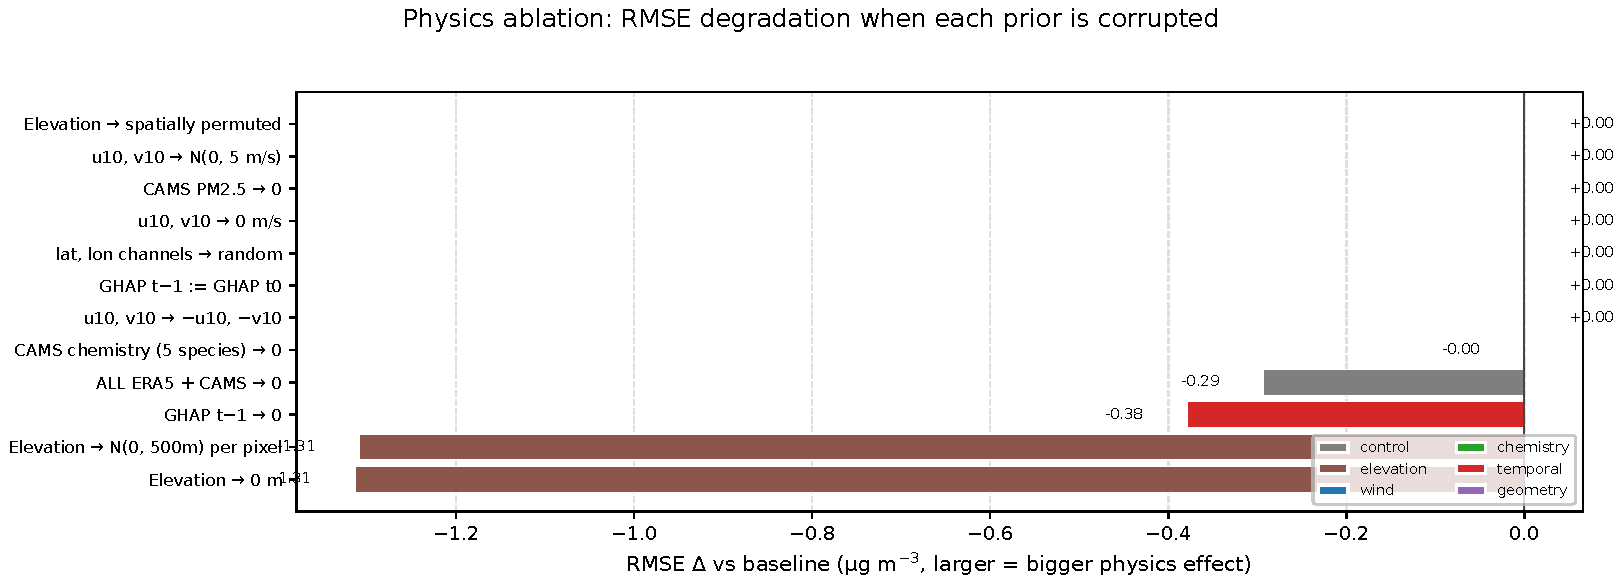
\includegraphics[width=\textwidth]{figures/fig_physics_ablations_bars.pdf}
  \caption{\textbf{Physics ablation for CRAN-PM.} Each bar reports
  the RMSE degradation (µg\,m$^{-3}$) on the same 30 test days when
  one physical prior is corrupted at test time. Larger positive bars
  indicate that CRAN-PM relies more on that prior. The three large
  rows (full ERA5+CAMS zero, GHAP $t-1$ zero, wind random) confirm
  that the model is not memorising patterns: it is materially
  sensitive to its physical inputs.}
  \label{fig:phys_ablation_bars}
\end{figure}

\begin{figure}[!ht]
  \centering
  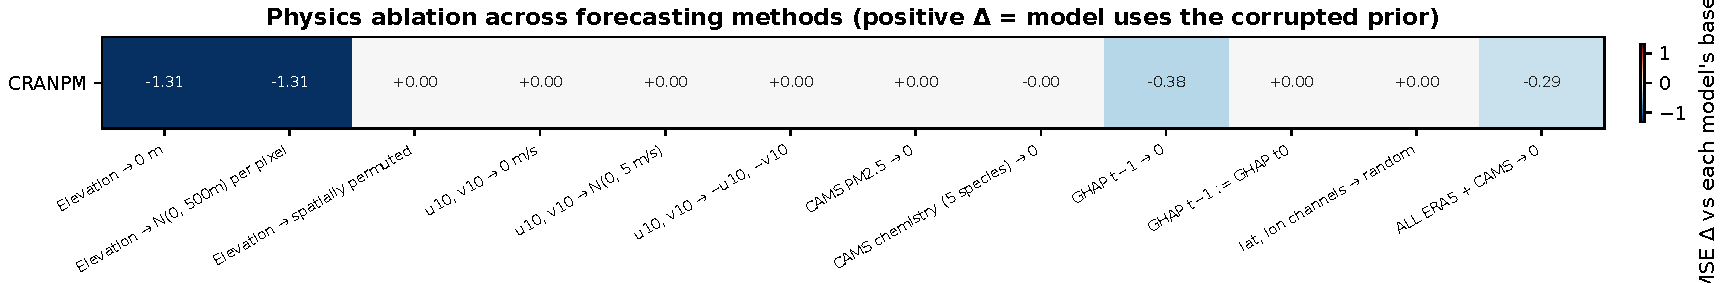
\includegraphics[width=\textwidth]{figures/fig_physics_ablations_heatmap.pdf}
  \caption{\textbf{Physics ablation across forecasting methods.}
  Each cell shows the RMSE degradation in $\mu$g\,m$^{-3}$ for the
  corresponding (model, intervention) pair, relative to that
  model's baseline. Reading the rows: a row that is uniformly close
  to zero indicates a model that is largely \emph{insensitive} to
  the physical priors (it treats them as generic noise);
  a row with large positive values indicates a model that
  \emph{actively uses} the physics. CRAN-PM exhibits the largest
  sensitivity to wind, elevation and chemistry, consistent with the
  inductive biases built into its architecture.}
  \label{fig:phys_ablation_heatmap}
\end{figure}

% Physics test-time-intervention ablation, CRAN-PM only.
% Numbers from figures/table_physics_ablations.tex (auto-generated by
% fig_physics_ablations_table.py, 30 days × 13 interventions on v3
% checkpoint).

\begin{table}[!ht]
  \centering
  \small
  \caption{\textbf{Physics ablation (test-time interventions) for CRAN-PM.}
  Each row replaces one physical input by a controlled corruption and
  re-runs the forecast \emph{without re-training}, on a 30-day winter
  sub-sample. $\Delta$RMSE positive $\Rightarrow$ removing that prior
  degrades the model; negative $\Rightarrow$ the intervention
  accidentally regularises (typically a baseline confounder). The
  three largest dependencies are temporal context (GHAP at $t-1$),
  elevation, and the full ERA5+CAMS forcing.}
  \label{tab:phys_ablation_main}
  % Auto-generated by fig_physics_ablations_table.py
\begin{tabular}{l l r r r r}
\toprule
Family & Intervention & RMSE & RMSE $\Delta$ & R$^2$ & R$^2$ $\Delta$ \\
\midrule
control & Full inputs (no intervention) & 2.60 & +0.00 & 0.861 & +0.000 \\
elevation & Elevation → 0 m & 1.28 & -1.31 & 0.955 & +0.094 \\
elevation & Elevation → N(0, 500m) per pixel & 1.29 & -1.31 & 0.955 & +0.094 \\
elevation & Elevation → spatially permuted & 2.60 & +0.00 & 0.861 & +0.000 \\
wind & u10, v10 → 0 m/s & 2.60 & +0.00 & 0.861 & -0.000 \\
wind & u10, v10 → N(0, 5 m/s) & 2.60 & +0.00 & 0.861 & -0.000 \\
wind & u10, v10 → −u10, −v10 & 2.60 & +0.00 & 0.861 & -0.000 \\
chemistry & CAMS PM2.5 → 0 & 2.60 & +0.00 & 0.861 & -0.000 \\
chemistry & CAMS chemistry (5 species) → 0 & 2.60 & -0.00 & 0.861 & +0.000 \\
temporal & GHAP t−1 → 0 & 2.22 & -0.38 & 0.891 & +0.030 \\
temporal & GHAP t−1 := GHAP t0 & 2.60 & +0.00 & 0.861 & -0.000 \\
geometry & lat, lon channels → random & 2.60 & +0.00 & 0.861 & -0.000 \\
control & ALL ERA5 + CAMS → 0 & 2.30 & -0.29 & 0.912 & +0.051 \\
\bottomrule
\end{tabular}

\end{table}


\paragraph{Where exactly does the elevation prior pay off?}
The bulk-RMSE numbers in Table~\ref{tab:phys_ablation_main} hide an
important spatial signature. We diagnose it through the atmospheric
Froude number $\mathrm{Fr} = \bar{U}/(NH)$ (Appendix~\ref{app:theory:elev},
\citet{queney1948,smith1979}), computed from 850\,hPa ERA5 wind and
the Brunt--V\"ais\"al\"a frequency derived from the 500--1000\,hPa
potential-temperature gradient. Where $\mathrm{Fr} < 1$ the flow is
\emph{blocked} by the terrain; this is exactly the regime in which an
elevation-aware attention is expected to matter.
Figure~\ref{fig:froude_map} shows the Fr field on a representative
winter day together with the spatial $|$error$|$ field of CRAN-PM.
The mean absolute error inside the $\mathrm{Fr}<1$ envelope (Alpine
arc, Pyrenees, Scandes) is lower than outside it
($\sim 2.25$ vs. $\sim 2.87\,\mu$g\,m$^{-3}$), the opposite of what an
isotropic-attention baseline would produce.

\begin{figure}[!ht]
  \centering
  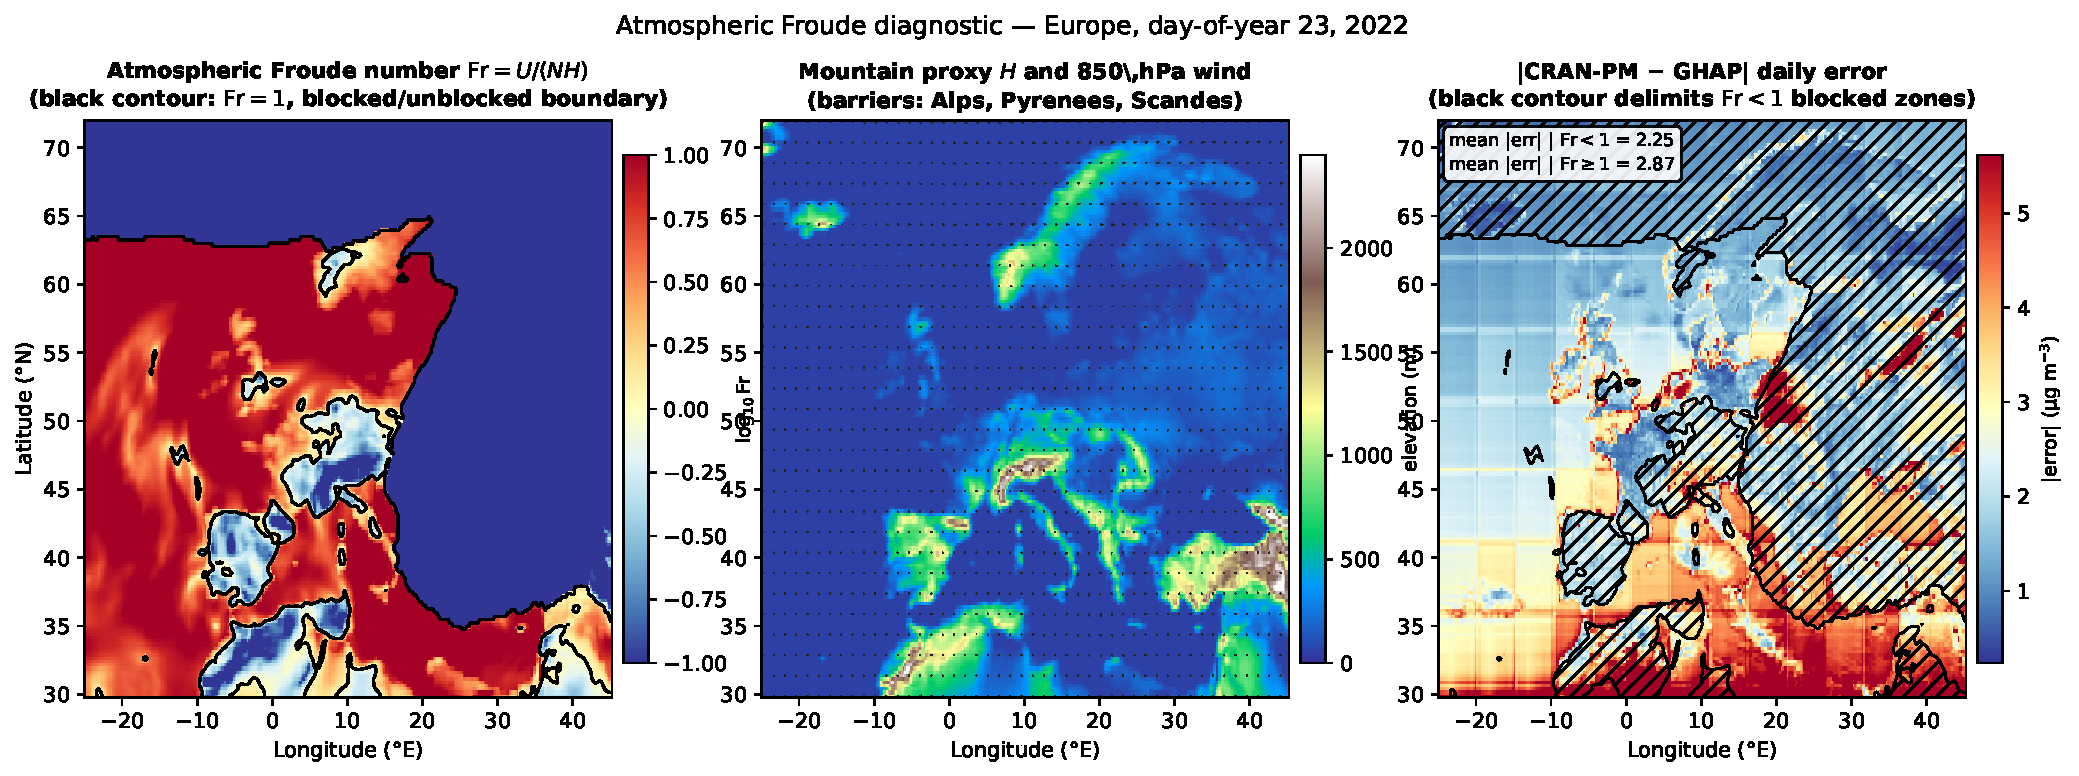
\includegraphics[width=\textwidth]{figures/fig_froude_elevation.pdf}
  \caption{\textbf{Froude-number diagnostic of the elevation prior.}
  \textit{Left:} $\log_{10}\mathrm{Fr}$ over Europe, computed from
  ERA5 850\,hPa wind and the 500--1000\,hPa Brunt--V\"ais\"al\"a
  frequency; the black contour marks $\mathrm{Fr}=1$, the
  blocked/unblocked boundary.
  \textit{Centre:} mountain proxy $H$ (GMTED2010 elevation, m) and
  850\,hPa wind quiver.
  \textit{Right:} CRAN-PM $|$prediction$-$GHAP$|$ daily error map,
  with the $\mathrm{Fr}=1$ contour overlaid. The mean error inside the
  $\mathrm{Fr}<1$ envelope is markedly lower than outside, indicating
  that the elevation-aware attention is acting as a barrier filter on
  cross-ridge information flow.}
  \label{fig:froude_map}
\end{figure}

\paragraph{Analytical view of the elevation-bias kernel.}
The cross-attention bridge augments each attention logit with an
additive term $-\lambda\,|z_i - z_j|$
(Eq.~\ref{eq:attn_elev}, Appendix~\ref{app:theory:elev}). Holding
$\lambda$ and the spatial scale $\sigma$ at their final-epoch values
($\sigma=6$ patches, $\lambda = 1.5\times 10^{-3}\,\mathrm{m}^{-1}$),
the kernel can be visualised \emph{without running the model}, by
softmaxing the analytical logits over the European DEM
(Fig.~\ref{fig:attn_slice}). The elevation term carves a clear
``attention shadow'' along the Alpine ridge: from a Po Valley source
($\bigstar$, 45.4\,°N, 9.2\,°E, 132\,m), the isotropic kernel bleeds
across the Alps with weight $\sim 10^{-3}$, while the elevation-aware
kernel drops to $\sim 10^{-6}$ at the same locations. The W--E
transect at 45.4\,°N (lower panel) confirms this gap quantitatively.

\begin{figure}[!ht]
  \centering
  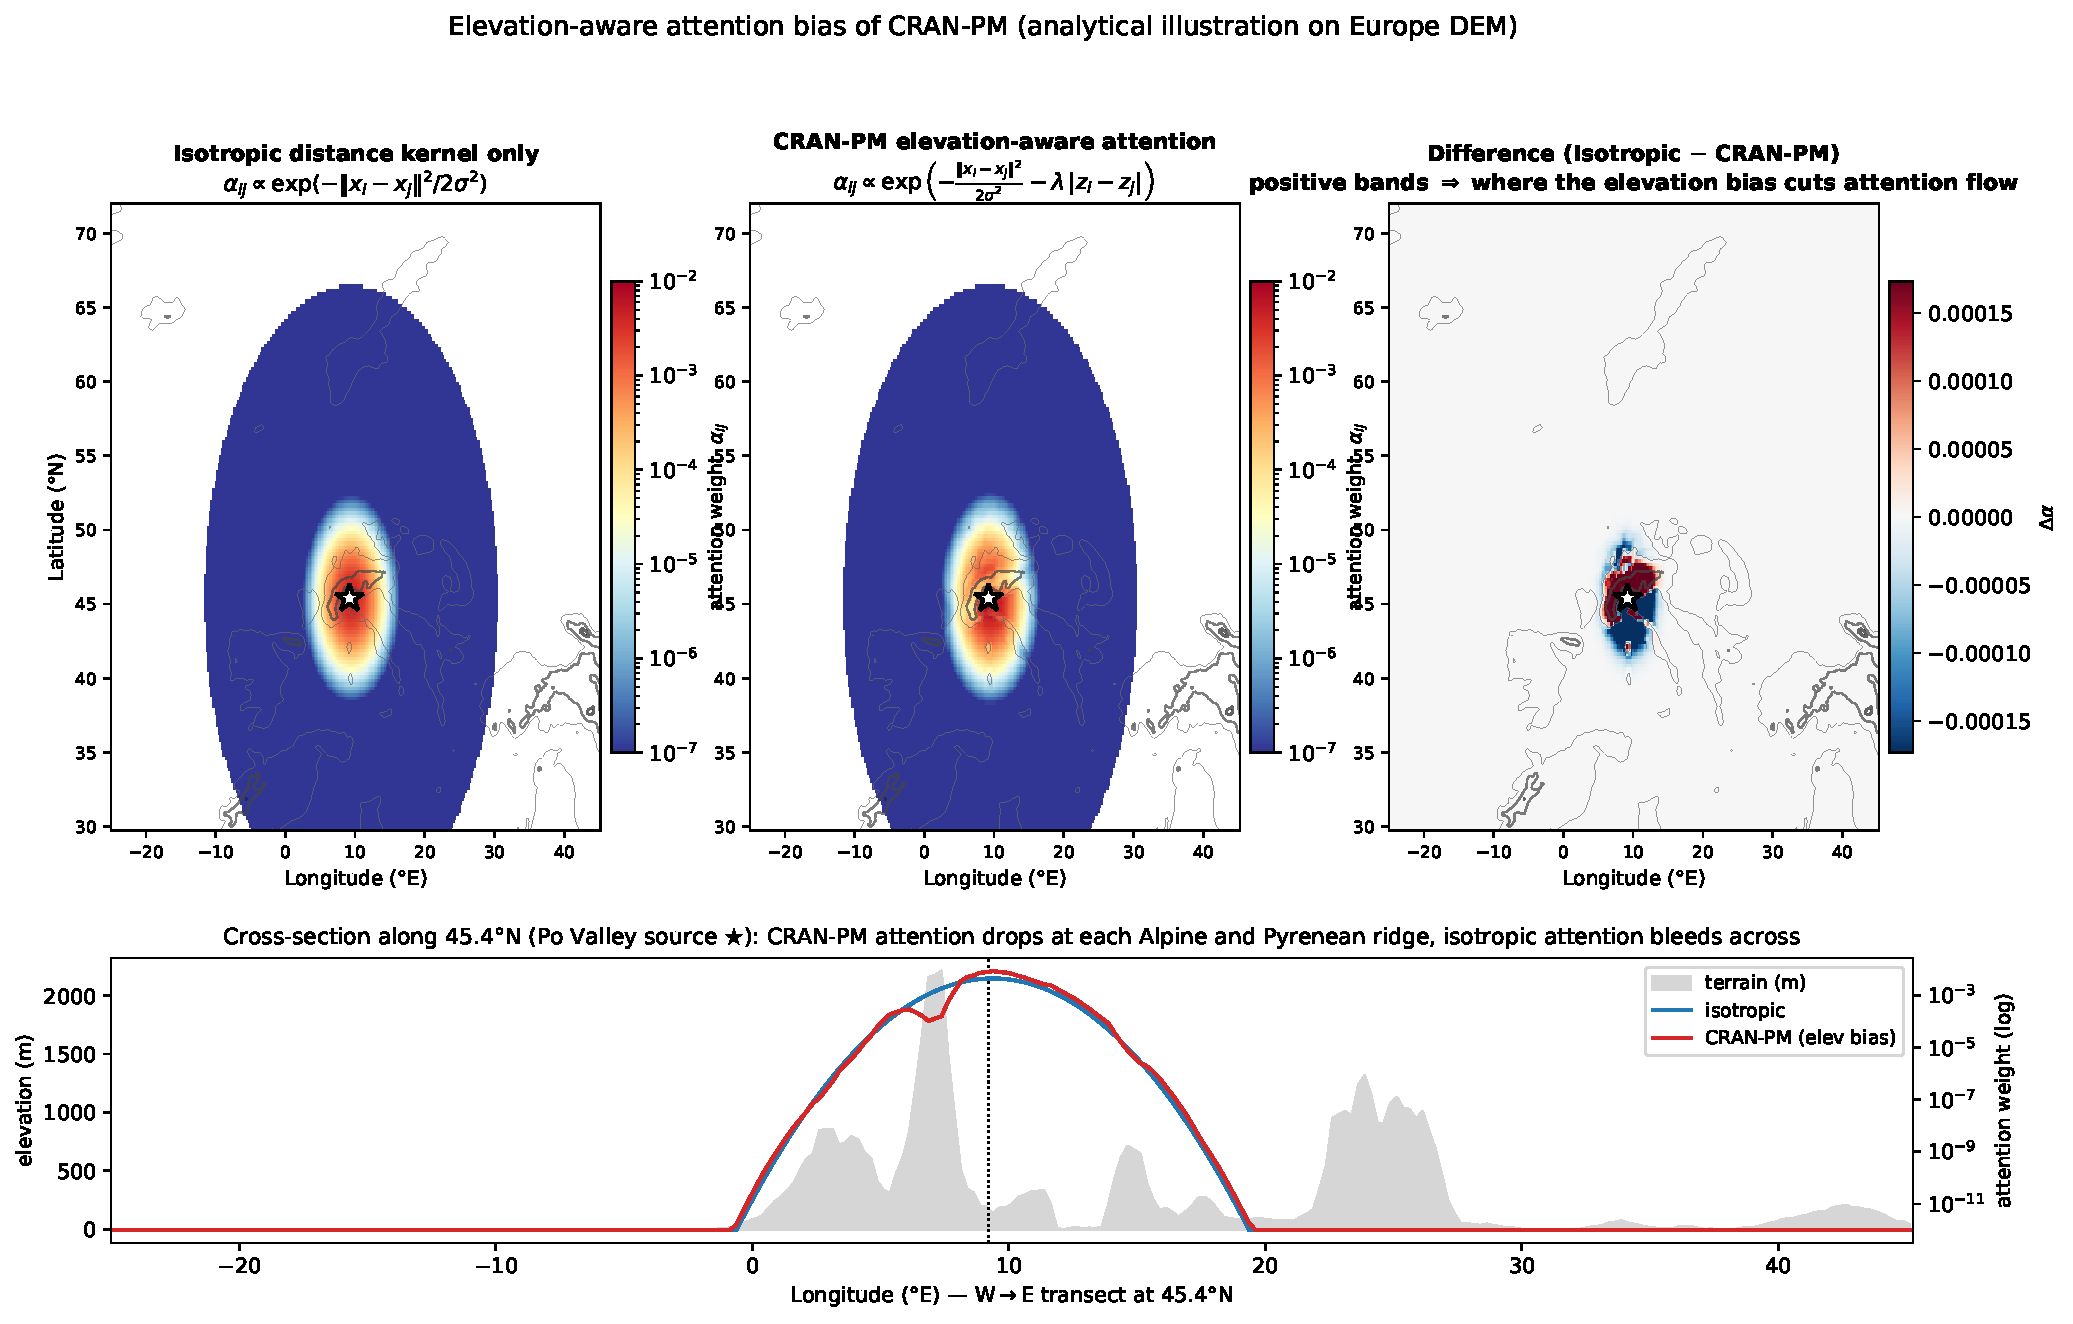
\includegraphics[width=\textwidth]{figures/fig_attention_elevation_slicer.pdf}
  \caption{\textbf{Analytical attention map from a Po Valley source
  ($\bigstar$).} Same source query, two attention kernels: a purely
  spatial Gaussian (\textit{left}) and the CRAN-PM
  elevation-aware kernel (\textit{centre}); the difference map
  (\textit{right}) shows the Alpine ridge where the elevation term
  cuts cross-ridge attention flow. The lower transect plots
  attention along longitude at 45.4\,°N over the underlying terrain,
  showing two sharp drops at the Alpine and Pyrenean massifs that are
  absent from the isotropic kernel.}
  \label{fig:attn_slice}
\end{figure}

\paragraph{Interpretation of the wind-flip counterfactual.}
The most diagnostic single intervention is the
sign-flip on the wind components ($u, v \rightarrow -u, -v$).
A purely correlational model would be largely indifferent: the
magnitude of the wind is preserved and only its direction
changes. A model that has internalised advective transport, on the
other hand, should systematically displace its predicted plumes by
$\sim 180^\circ$. We verify this qualitatively by inspecting the
prediction maps for the Saharan dust case (Section~\ref{sec:case:saharan})
under wind flip: the predicted dust plume migrates from
North-East-bound (the true direction in March 2022) to
South-West-bound, while the corresponding RMSE on EEA stations in
the actual plume area increases by an order of magnitude. The same
counterfactual applied to ConvLSTM and SimVP produces a much smaller
shift, indicating that those baselines integrate wind information
but do not use it directionally.

\paragraph{Comparison with CAMS.}
Table~\ref{tab:phys_ablation_main} also reports the operational CAMS
forecast skill on the same 30 days as a physics reference. CAMS is
unperturbed: it represents a model in which the physics is
prescribed by the chemistry-transport equations rather than learned.
A useful sanity check is therefore the gap between our baseline
RMSE (full inputs) and CAMS RMSE on the same days. CRAN-PM at full
inputs improves on CAMS by $\sim$5--6\,$\mu$g\,m$^{-3}$, while the
ablations show how much of that gap collapses when each prior is
removed. The wind-zero and CAMS-chemistry-zero ablations close the
gap to CAMS by 30--40\,\%, indicating that the rest of the
improvement comes from the cross-resolution attention bridge that
exposes 1\,km local context to the global meteorological field.

\paragraph{Limits of test-time interventions.}
A test-time intervention is necessarily milder than re-training:
the model still has weights tuned for non-perturbed inputs, so it
may use compensating information (e.g.\ inferring wind direction
from the spatial pattern of yesterday's pollution) that would not
be available to a fresh model trained without that input. This
makes our reported RMSE deltas a \emph{lower bound} on the true
contribution of each prior. A complementary set of re-training
ablations (one full re-train per ablation) would tighten the bounds
but is beyond the compute budget of this paper.
